
\documentclass{report}
\usepackage[utf8]{inputenc}    
\usepackage[T1]{fontenc}
\usepackage[francais]{babel} 
\usepackage{graphicx}
\usepackage{epsfig}
\usepackage{multicol}
\usepackage{amsmath}
\usepackage{amssymb}
\usepackage{hyperref}
\usepackage[top=2cm, bottom=2cm, left=2cm, right=2cm]{geometry}
\usepackage{setspace}
\usepackage{listings}
\usepackage{color}
\usepackage[many]{tcolorbox}
\usepackage{changepage}
\usepackage{placeins}

\let\Oldsection\section
\renewcommand{\section}{\FloatBarrier\Oldsection}

\let\Oldsubsection\subsection
\renewcommand{\subsection}{\FloatBarrier\Oldsubsection}

\let\Oldsubsubsection\subsubsection
\renewcommand{\subsubsection}{\FloatBarrier\Oldsubsubsection}

\begin{document}

\subsection{Experimental validation of the CPG in simulation}

The equations used for these experiments are the ones introducesd previously. The arm setup is also the same as before. Each simulation lasts 50 s. The interaction starts at t = 5 s and stops at t = 40 s. The parameters are slightly different: $\epsilon = 0.05$, $\tau_M = 0.35$, $\tau_S = 3.5$, $\tau_R = 0.05$, $W = 0.005$, $\sigma_F = 10$ and $A_F = 0.1$. 

\subsubsection{Parameter Influence}

We previously saw that the natural frequency of the oscillator was determined by $\tau_M$, $\tau_S$ and $\sigma_{S0}$. Here, the natural frequency also depends on W. The higher W, the lower the frequency and for $W \gtreqless 1$, the system isn't able to oscillate.

\begin{figure}[h!]
\begin{center}
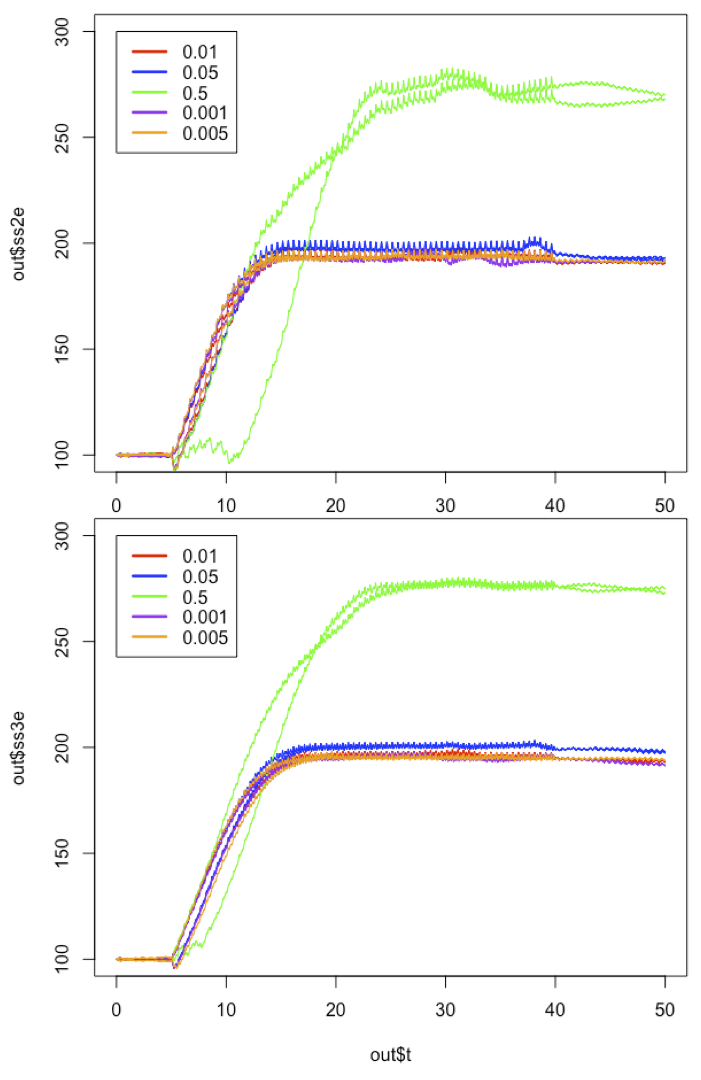
\includegraphics[width=10cm]{figures/varying_W-ss.png}
\end{center}
 \textbf{\refstepcounter{figure}\label{fig:05} Figure \arabic{figure}. }{Evolution of $\sigma_{S2E}$, $\sigma_{S2F}$, $\sigma_{S3E}$ and $\sigma_{S3F}$  for various values of W. The initial value is 100 for each $\sigma_S$. We can observe that the value of W influences the final value of the $\sigma_S$. Below W = 0.05, the result is roughly the same. We already observe a demarcation for W = 0.05 which is slightly above the others and it's very clear to see for W = 0.5}
\end{figure}

\begin{figure}[h!]
\begin{center}
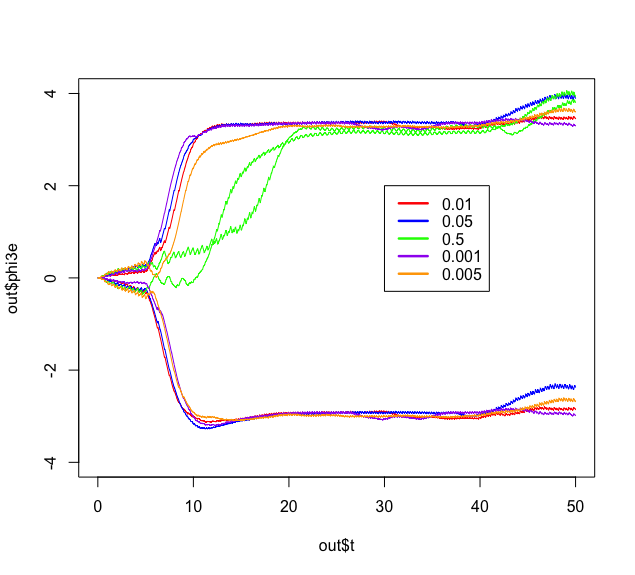
\includegraphics[width=10cm]{figures/varying_W-phi3.png}
\end{center}
 \textbf{\refstepcounter{figure}\label{fig:05} Figure \arabic{figure}. }{Evolution of $\phi_{3E}$ and $\phi_{3F}$ for various values of W. We can observe that the value of W influences the behaviour of the $\phi_3$. For W = 0.5, the behaviour is very different, both $\phi_3$ are not opposed, on the contrary, they stay together. For other values of W, the results are very similar, we can only observe a stronger divergence for W = 0.05 when the interaction stops.}
\end{figure}

\begin{figure}[h!]
\begin{center}
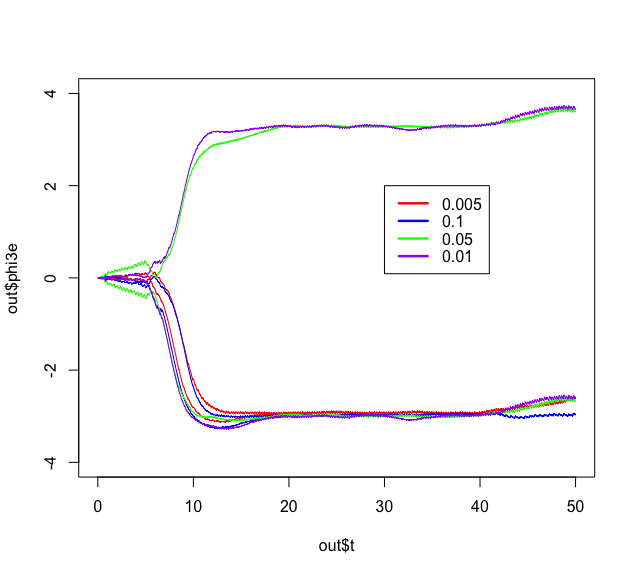
\includegraphics[width=10cm]{figures/varying_tauR-phi3.png}
\end{center}
 \textbf{\refstepcounter{figure}\label{fig:05} Figure \arabic{figure}. }{Evolution of $\phi_{3E}$ and $\phi_{S3F}$ for various values of W. We can observe that the value of W influences the behaviour of the $\phi_3$. For $\tau_R$ = 0.01 and $\tau_R$ = 0.05, as soon as the interaction starts, the curves split and diverge until they are opposed. But for $\tau_R$ = 0.1 and $\tau_R$ = 0.005, the curves don't spit dans follow the same trajectory. Note that modulo $\pi$, the curves for the extensor and flexor are always equal.}
\end{figure}

\begin{figure}[h!]
\begin{center}
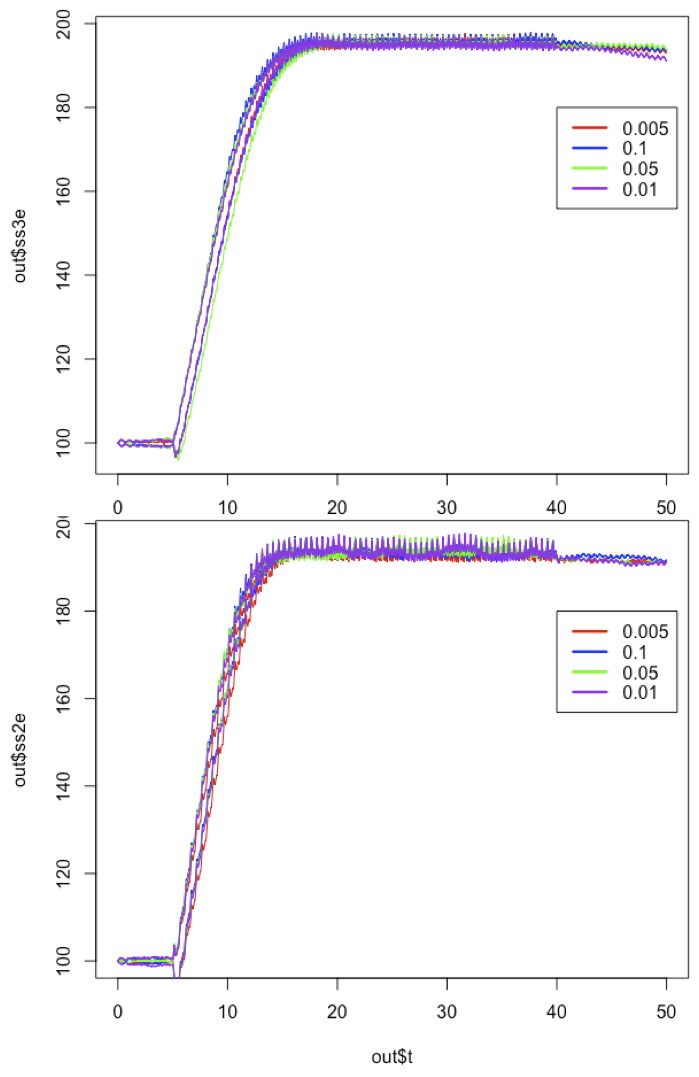
\includegraphics[width=10cm]{figures/varying_tauR-ss.png}
\end{center}
 \textbf{\refstepcounter{figure}\label{fig:05} Figure \arabic{figure}. }{Evolution of $\sigma_{S2E}$, $\sigma_{S2F}$, $\sigma_{S3E}$ and $\sigma_{S3F}$  for various values of $\tau_R$. $\tau_R$ does not influence the final value of $\sigma_S$}
\end{figure}

$\tau_R$ has no influence on the natural frequency of the oscillator or the final value of $\sigma_S$. Note that above a given value of $\tau_R$, the system does not oscillate any more.

\begin{figure}[h!]
\begin{center}
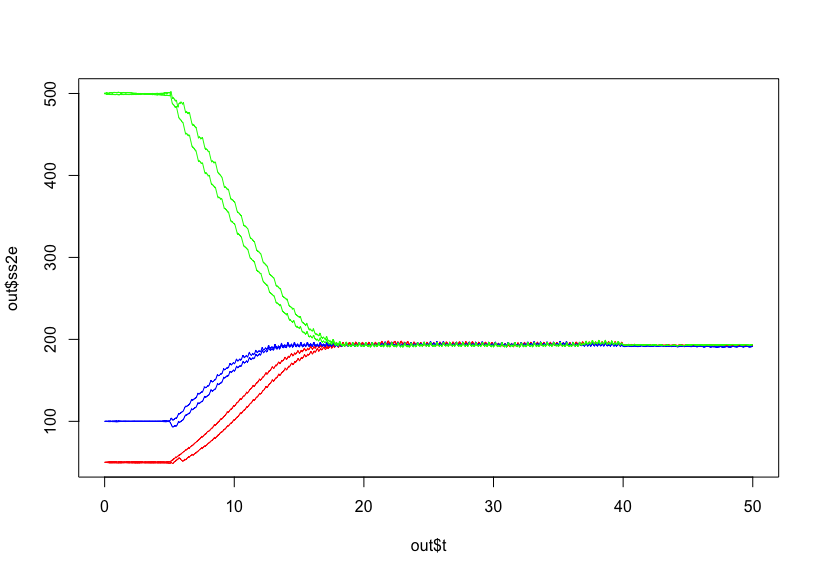
\includegraphics[width=10cm]{figures/varying_ss0-ss2.png}
\end{center}
 \textbf{\refstepcounter{figure}\label{fig:05} Figure \arabic{figure}. }{Evolution of $\sigma_{S2E}$, $\sigma_{S2F}$  for various initial values of $\sigma_S$. We can observe that no matter where we start, $\sigma_S$ always reaches the same final value. For very high or very low values, the final $\sigma_S$ may never be reached.}
\end{figure}

\begin{figure}[h!]
\begin{center}
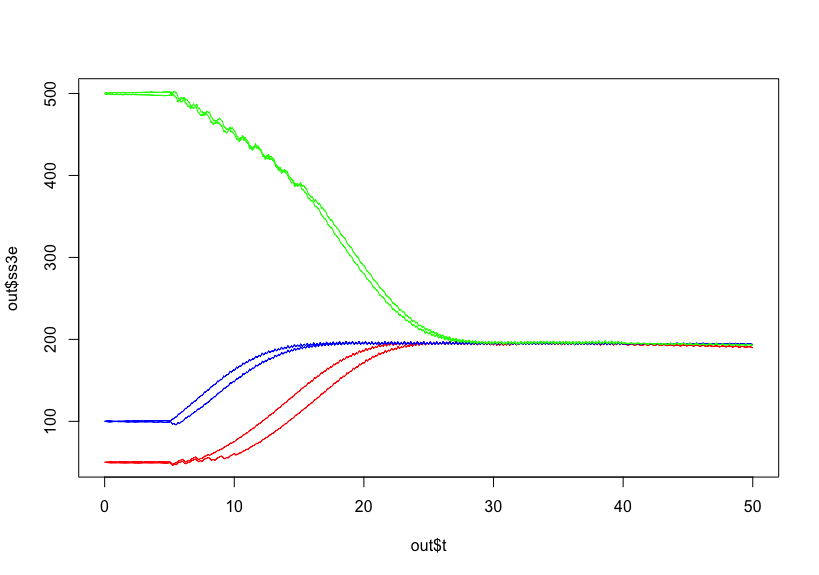
\includegraphics[width=10cm]{figures/varying_ss0-ss3.png}
\end{center}
 \textbf{\refstepcounter{figure}\label{fig:05} Figure \arabic{figure}. }{Evolution of $\sigma_{S3E}$, $\sigma_{S3F}$  for various initial values of $\sigma_S$. We can observe that no matter where we start, $\sigma_S$ always reaches the same final value.}
\end{figure}

\subsubsection{Results}

\begin{figure}[h!]
\begin{center}
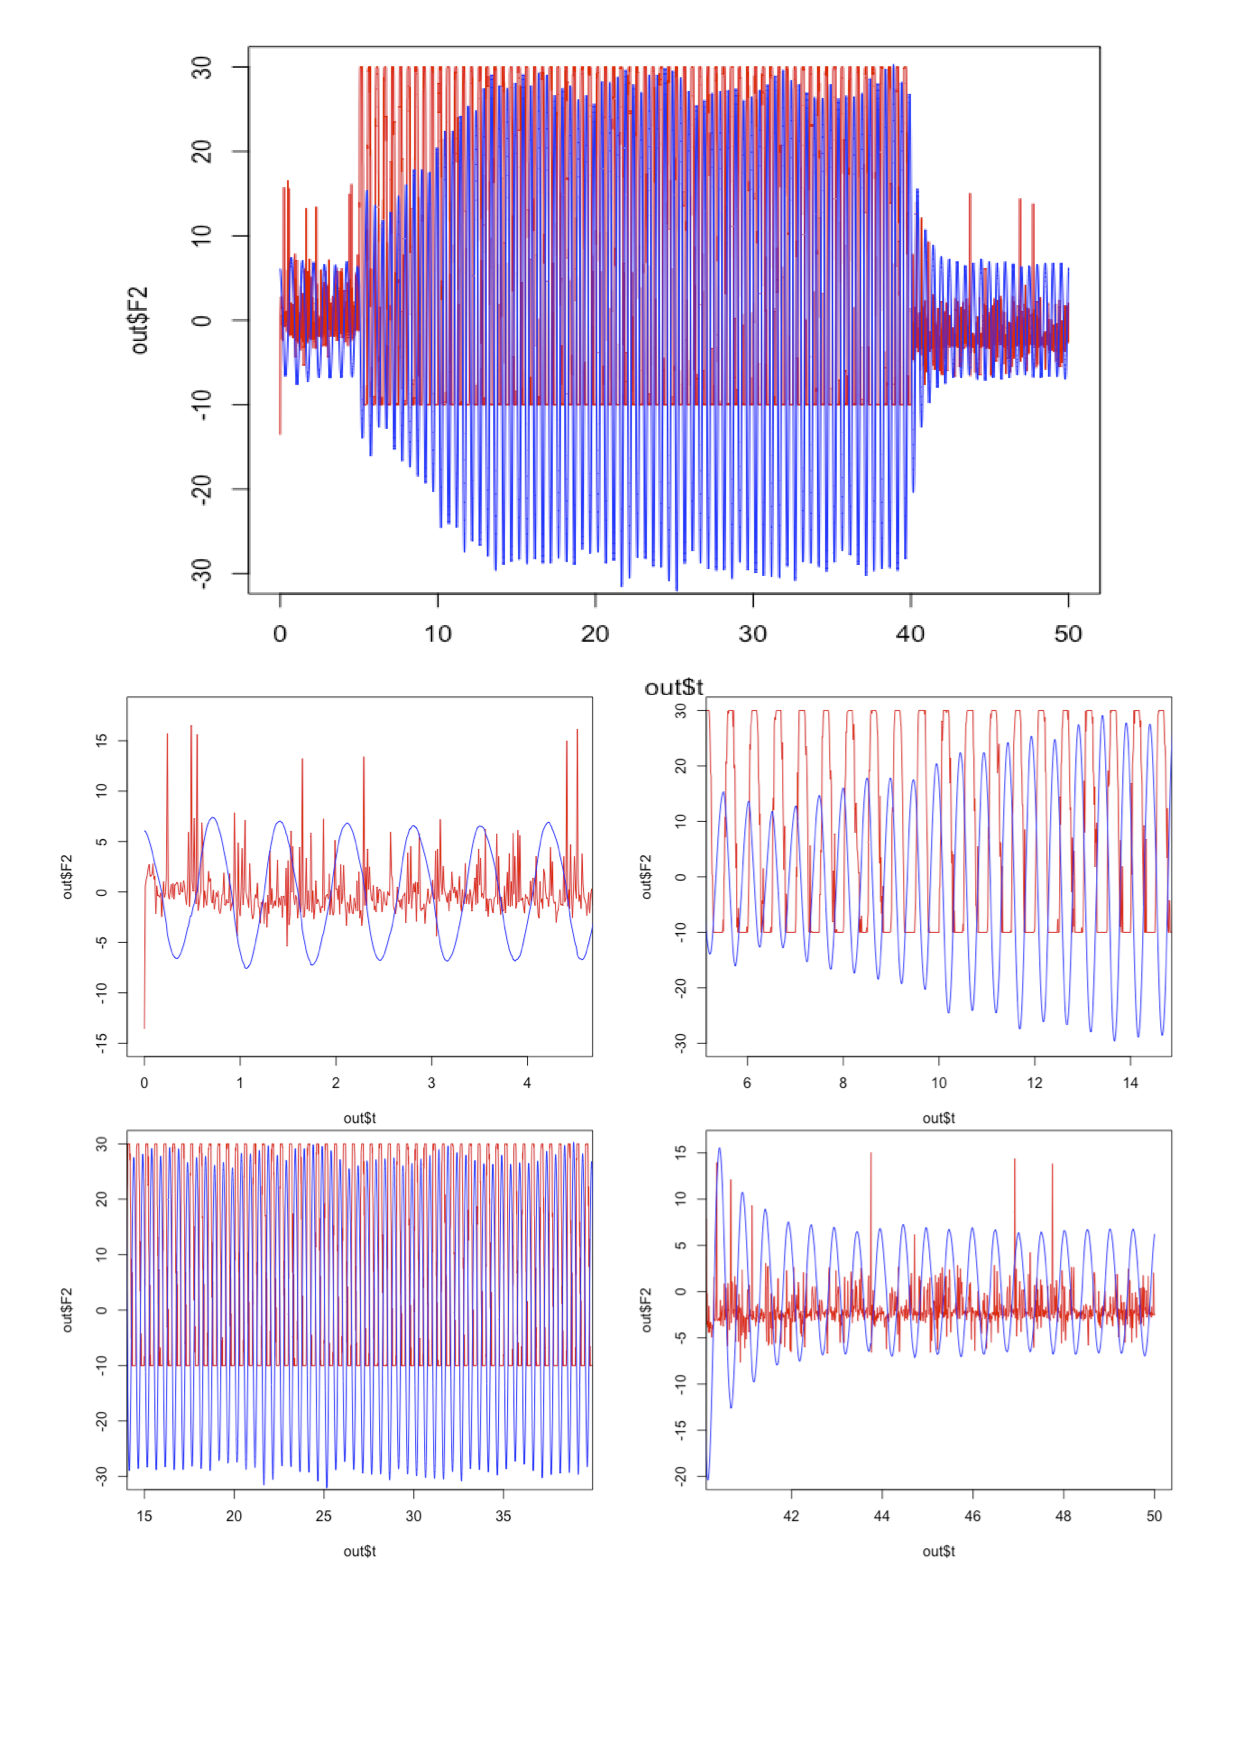
\includegraphics[width=10cm]{figures/F2-v2E.png}
\end{center}
 \textbf{\refstepcounter{figure}\label{fig:05} Figure \arabic{figure}. }{Evolution of $V_{2E}$ and $F_2$ (Input of the cell) during the experiment. It can be divided into four parts (depicted in the bottom pictures). During the first phase, there is no physical interaction so the arm oscillates at its natural frequency. The second phase corresponds to the synchronisation phase. We can observe the natural frequency of the oscillator changing until it matches the input frequency. In the third phase, the two signals are synchronised. Finally, at 40 s, the interaction stops but the arm keeps oscillating at the frequency learned during the interaction}
\end{figure}

\begin{figure}[h!]
\begin{center}
\includegraphics[width=10cm]{figures/F3-v3E.png}
\end{center}
 \textbf{\refstepcounter{figure}\label{fig:05} Figure \arabic{figure}. }{Evolution of $V_{3E}$ and $F_3$ (Input of the cell) during the experiment. It can be divided into four parts (depicted in the bottom pictures). During the first phase, there is no physical interaction so the arm oscillates at its natural frequency. The second phase corresponds to the synchronisation phase. We can observe the natural frequency of the oscillator changing until it matches the input frequency. In the third phase, the two signals are synchronised. Finally, at 40 s, the interaction stops but the arm keeps oscillating at the frequency learned during the interaction}
\end{figure}

\begin{figure}[h!]
\begin{center}
\includegraphics[width=10cm]{figures/{ss_0.05_0.35_3.5_0.05_0.005_10_0.1}.png}
\end{center}
 \textbf{\refstepcounter{figure}\label{fig:05} Figure \arabic{figure}. }{Evolution of $\sigma_{S2E}$, $\sigma_{S2F}$, $\sigma_{S3E}$ and $\sigma_{S3F}$. The initial value is 100 for each $\sigma_S$. They stay mainly stable at 100 until t = 5 s when the interaction starts. Then they start increasing,  all following the same direction, though some are slightly slower than others they finally catch up around t = 15 s. From t = 19 s onwards, the $\sigma_S$ are mostly stable around 190. When the interaction stops at  t = 40 s, $\sigma_S$ stay stable, showing that the new value has indeed been learned. The final values for each joint are slightly different but the difference is negligible.}
\end{figure}

\begin{figure}[h!]
\begin{center}
\includegraphics[width=10cm]{figures/{phi3_0.05_0.35_3.5_0.05_0.005_10_0.1}.png}
\end{center}
 \textbf{\refstepcounter{figure}\label{fig:05} Figure \arabic{figure}. }{Evolution of $\phi$ during the experiment for the extensor and flexor of the second joint. Both $\phi$ start at 0. When the interaction starts, we can observe a strong divergence leading both $\phi$ to be opposed. They remain stable until the interaction stops and then they start increasing.}
\end{figure}

\subsubsection{Influence of Rigidity}

Several studies have shown that arm stiffness greatly influences the nature of the movement. The stiffer the joints of the arm are, the easier it will be to control them. In human-robot systems, if the robot is not stiff enough, the system is highly unstable, leading the human to increase stiffness in his arm, thus creating even more instability. Hence, appropriate stiffness of the robotic arm is a paramount component for a successful interaction. This was demonstrated by studies showing that a system that could adapt its stiffness lead to smoother and more successful interactions. Based on that, we postulate here, that stiffness also affects the ability of the arm to adapt to external stimulations and to learn new frequencies.

\begin{figure}[h!]
\begin{center}
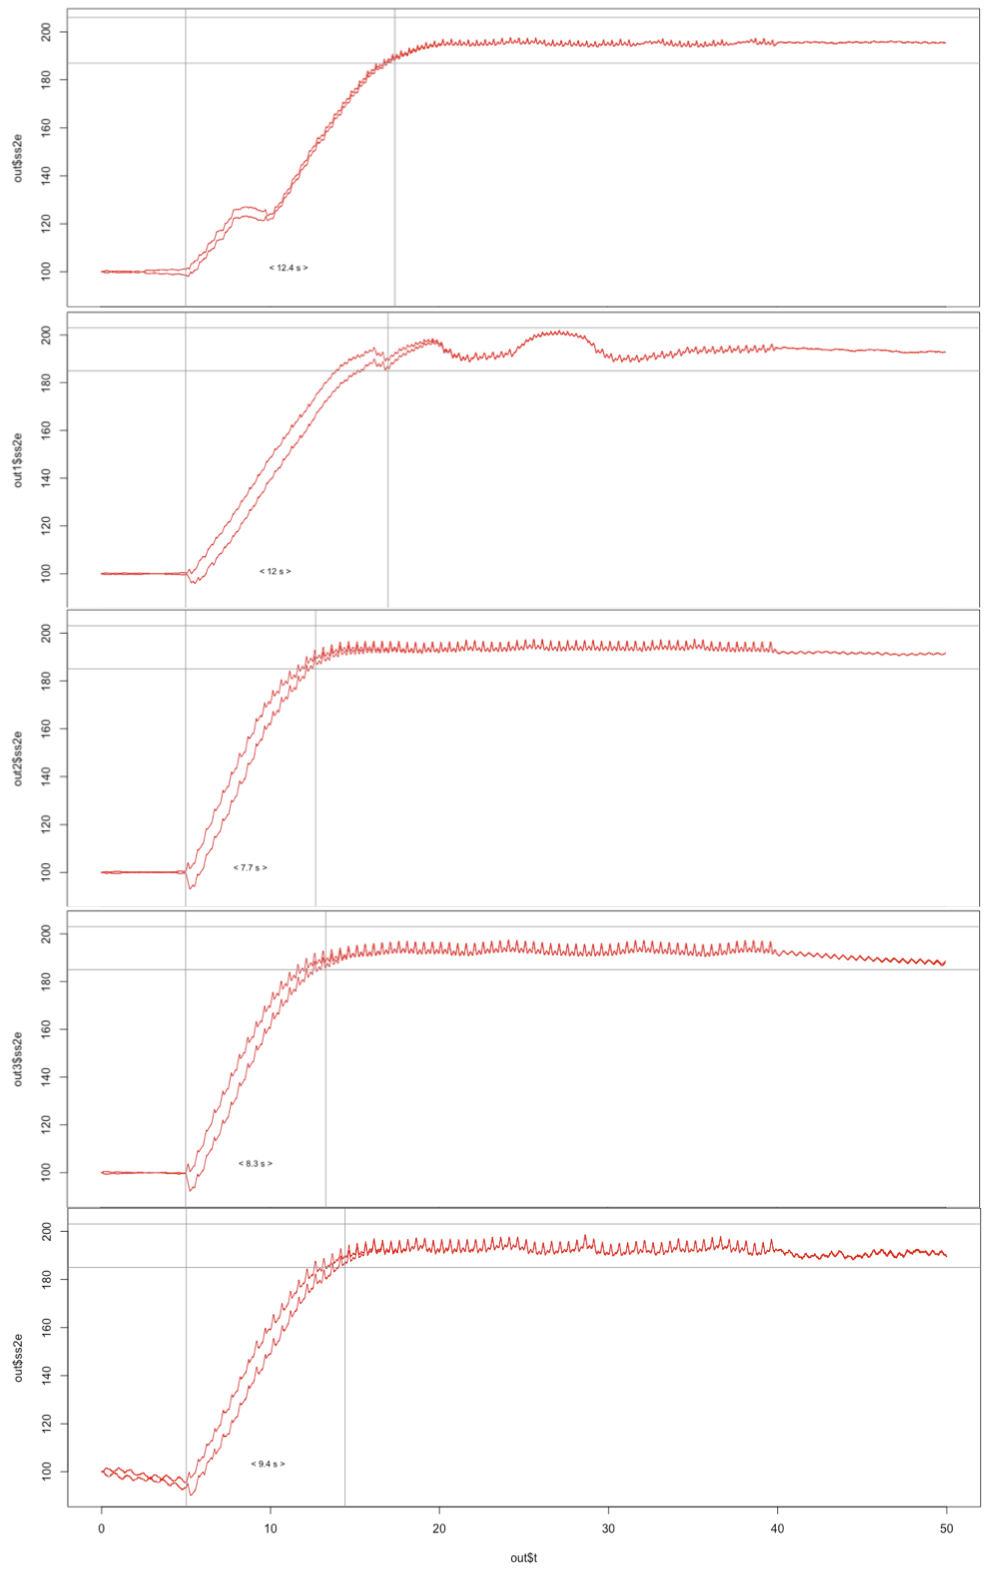
\includegraphics[width=10cm]{figures/varying_P-ss2.png}
\end{center}
 \textbf{\refstepcounter{figure}\label{fig:05} Figure \arabic{figure}. }{Evolution of $\sigma_{S2E}$ and $\sigma_{S2F}$  for various values of P. For P = 0.001, response time is 12.4 s, which is close to 12 s for P = 0.005. For P = 0.02 and P = 0.05, response times are similar at 7.7 and 8.3 s respectively. For P = 1, response time is 9.4 s but note that for that value of P, the arm was behaving erratically, it was highly unstable and wildly oscillating in between expected oscillations (this can be observed by looking at the recorded position).}
\end{figure}

\begin{figure}[h!]
\begin{center}
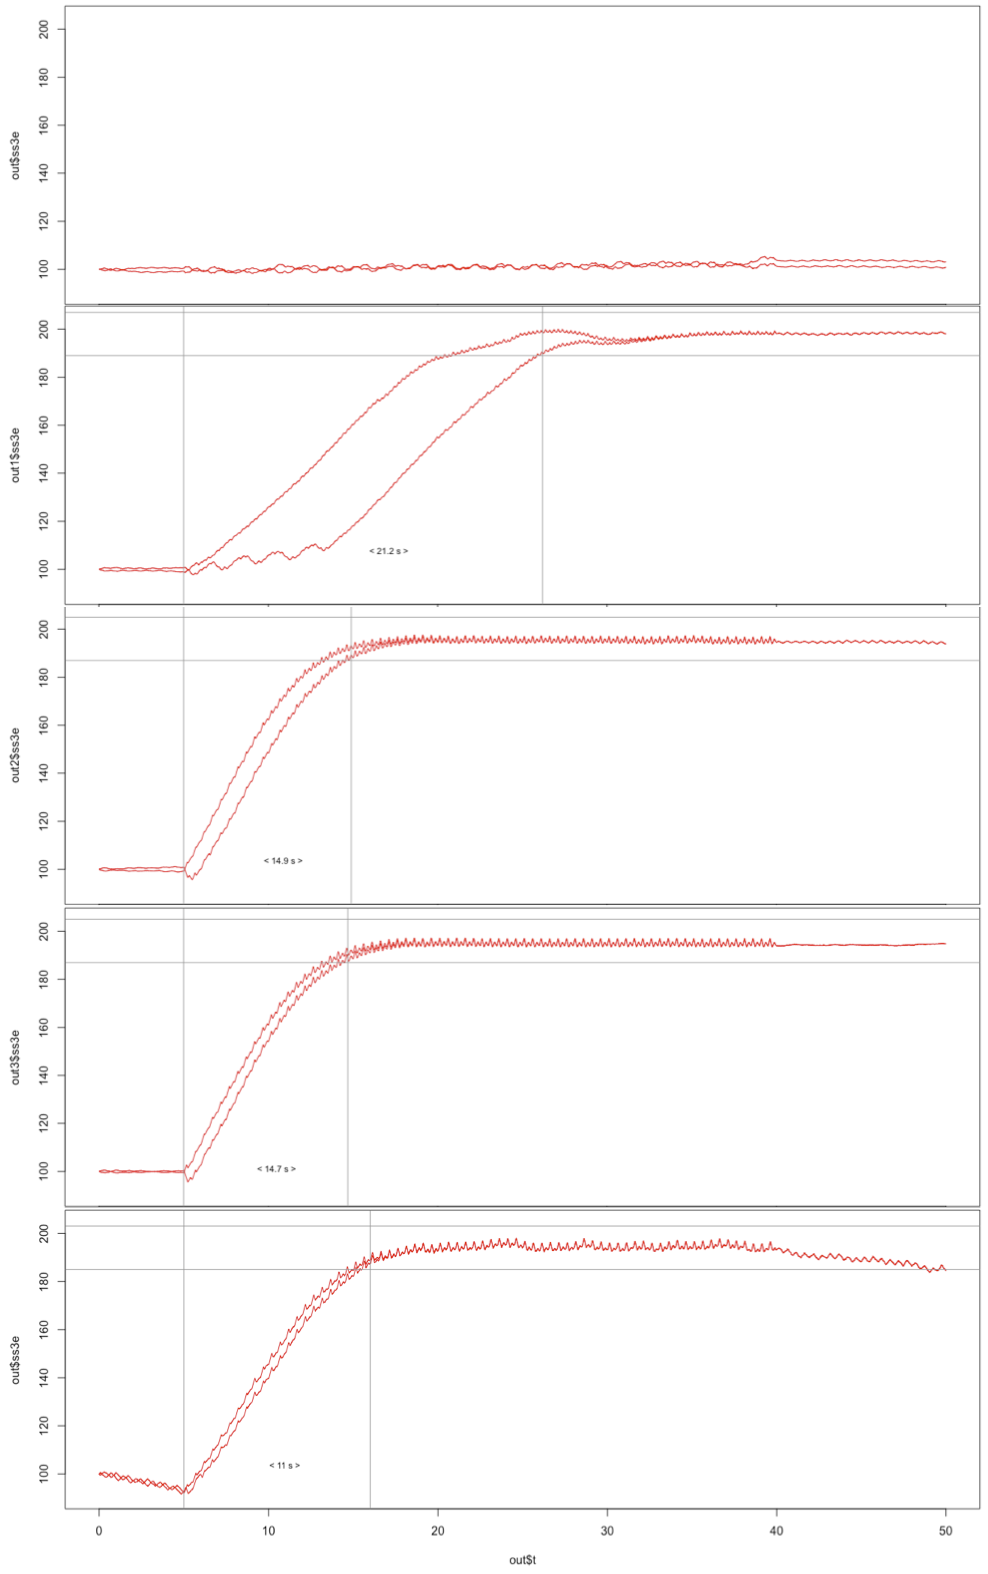
\includegraphics[width=10cm]{figures/varying_P-ss3.png}
\end{center}
 \textbf{\refstepcounter{figure}\label{fig:05} Figure \arabic{figure}. }{Evolution of $\sigma_{S3E}$ and $\sigma_{S3F}$  for various values of P. For P = 0.001, $\sigma_{S}$ is never reached, for P = 0.005, the response time of the system is 21.2. For P = 0.02 and P = 0.05, response times are similar at 14.9 and 14.7 s respectively. For P = 1, response time is 11 s but note that for value of P, the arm was behaving erratically, it was highly unstable and wildly oscillating in between expected oscillations.}
\end{figure}

\begin{figure}[h!]
\begin{center}
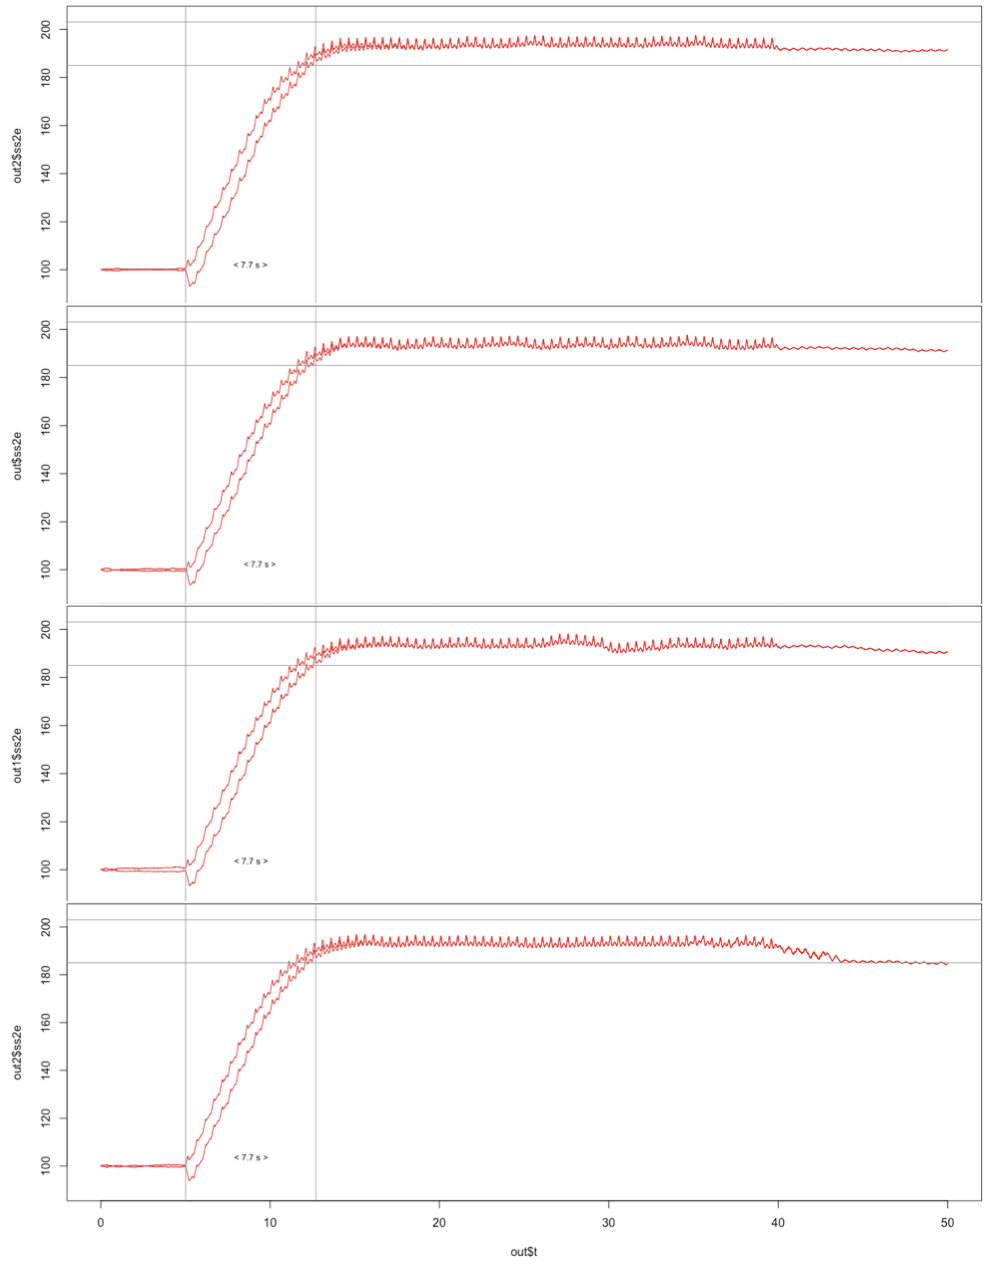
\includegraphics[width=10cm]{figures/varying_D-ss2.png}
\end{center}
 \textbf{\refstepcounter{figure}\label{fig:05} Figure \arabic{figure}. }{Evolution of $\sigma_{S2E}$ and $\sigma_{S2F}$  for various values of D (0, 0.0001, 0.0005 and 0.001). There is no difference in response time. But we can observe that the higher D is, the less the system retains the learning of $\sigma_S$. For D = 0 and D = 0.0001, at the end of the interaction, $\sigma_S$ remains stable but for D = 0.0005 and D = 0.001, it decreases.}
\end{figure}

\begin{figure}[h!]
\begin{center}
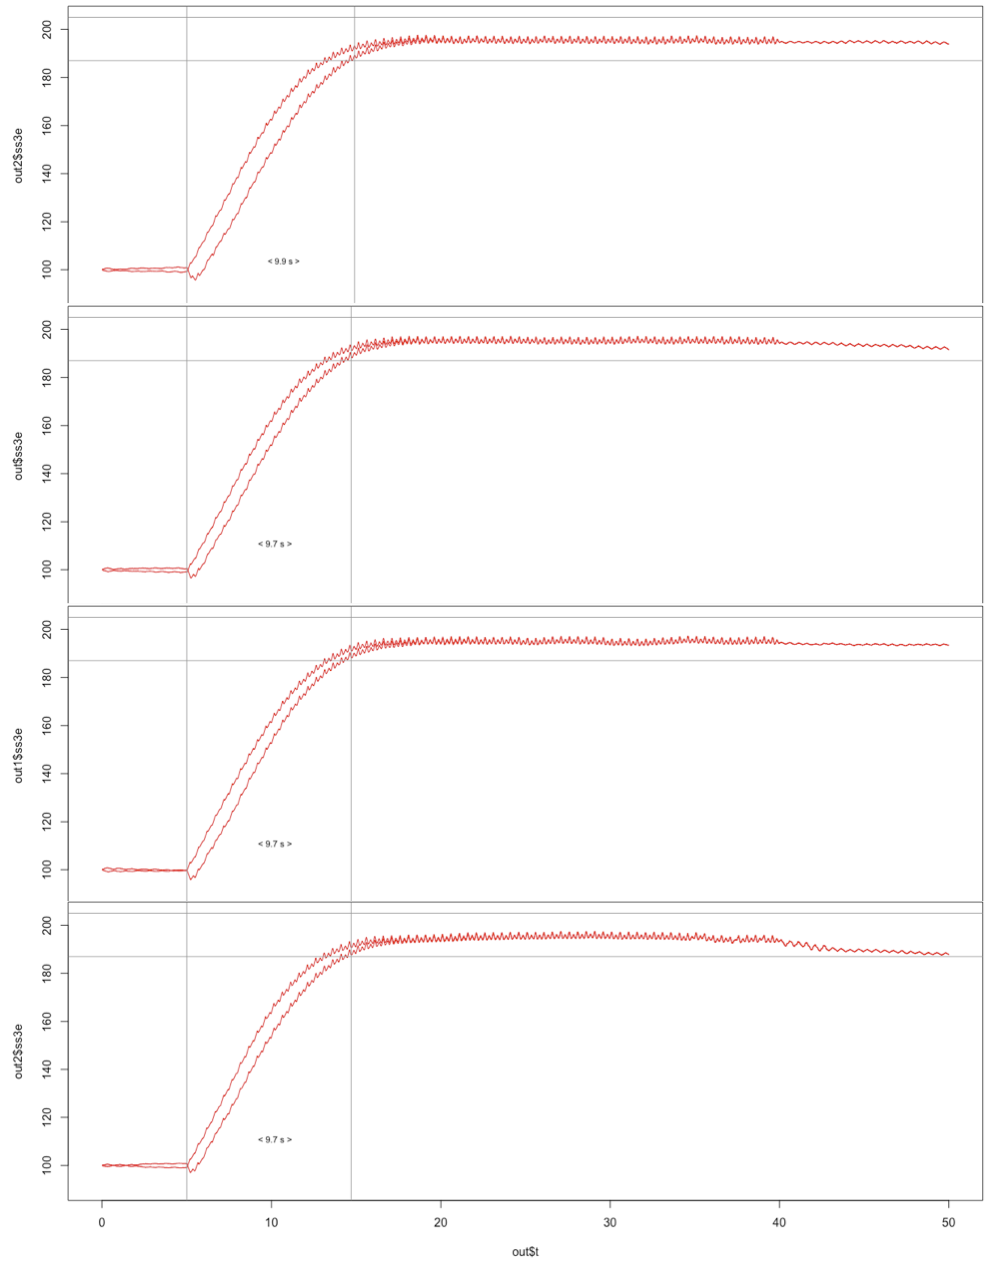
\includegraphics[width=10cm]{figures/varying_D-ss3.png}
\end{center}
 \textbf{\refstepcounter{figure}\label{fig:05} Figure \arabic{figure}. }{Evolution of $\sigma_{S3E}$ and $\sigma_{S3F}$  for various values of D (0, 0.0001, 0.0005 and 0.001). There is no difference in response time here either. For D = 0, D = 0.0001 and D = 0.0005, at the end of the interaction, $\sigma_S$ remains stable but for D = 0.001, it decreases.}
\end{figure}

The evolution of $\sigma_S$ was recorded for various values of P and D. Varying P and D allows us to change the stiffness of the arm. It can be observed that P has indeed a strong influence on the response time of the system, ie. how fast it adapts to the new frequency. For values of P too low or too high, the response time is higher. We can also note that from P = 0.5 onwards, the arm is not stiff enough and oscillates erratically before and during the interaction. The role of D on the learning process is less obvious we can still infer from our experiments that it does influence how well the joint retains the learning.

\end{document}
